% Common preamble for PIGMIE patent figures (A4).
% Drawing conventions:
%   - A4 portrait
%   - Sans-serif throughout (Helvetica)
%   - "Fig. N" sentence-case caption near top
%   - Page "N/total" at top centre
%   - Reference numerals outside boxes via leader lines
%   - ALL CAPS labels in component boxes
%   - Reactor uses north-east-lines hatched fill
%   - Scene uses double-line border
%   - Module enclosures use dashed line with internal numeral

\documentclass[a4paper,10pt]{article}
\usepackage[top=2.5cm,bottom=1.0cm,left=2.5cm,right=1.5cm]{geometry}
\usepackage[T1]{fontenc}
\usepackage{helvet}
\renewcommand{\familydefault}{\sfdefault}
\usepackage{amsmath,amssymb,bm}
\usepackage{tikz}
\usetikzlibrary{shapes,shapes.geometric,shapes.misc,arrows.meta,positioning,fit,calc,backgrounds,decorations.pathreplacing,decorations.markings,patterns}
\pagestyle{empty}
\setlength{\parindent}{0pt}

\tikzset{
  % Component box: ALL CAPS label inside, no numeral inside
  cbox/.style={draw, rectangle, minimum height=1.0cm, minimum width=2.4cm,
               align=center, line width=0.5pt, font=\small},
  cbox-tall/.style={cbox, minimum height=1.6cm},
  cbox-wide/.style={cbox, minimum width=3.0cm},
  cbox-narrow/.style={cbox, minimum width=1.8cm, font=\footnotesize},
  % Reactor / physical medium: hatched fill
  reactor/.style={cbox, pattern=north east lines, pattern color=black!70},
  % Scene: double-line border
  scenebox/.style={cbox, double, double distance=1.2pt, line width=0.4pt},
  % Module / sub-module enclosure
  enclosure/.style={draw, rectangle, dashed, line width=0.4pt, inner sep=10pt, rounded corners=2pt},
  enclosure-solid/.style={draw, rectangle, line width=0.5pt, inner sep=10pt, rounded corners=2pt},
  % Arrows
  flowarr/.style={-Latex, line width=0.5pt, font=\scriptsize},
  flowbi/.style={Latex-Latex, line width=0.5pt, font=\scriptsize},
  flowarr-fb/.style={-Latex, line width=0.5pt, dashed, font=\scriptsize},
  % Reference numeral leader-line endpoint and label
  refnum/.style={font=\footnotesize, inner sep=1pt},
  leader/.style={line width=0.4pt, -Latex},
  % Caption banner
  figcap/.style={font=\bfseries\large}
}

% Helper: figure header (page number + Fig. N caption)
\newcommand{\figheader}[3]{%
  % #1 = page number (e.g. "1"), #2 = total pages, #3 = figure label (e.g. "1" or "4A")
  \noindent\hfill\small #1/#2\hfill\null\par
  \vspace{0.2cm}
  \begin{center}\bfseries Fig.\ #3\end{center}
  \vspace{0.2cm}
}


\begin{document}

\figheader{3}{7}{3}

\begin{center}
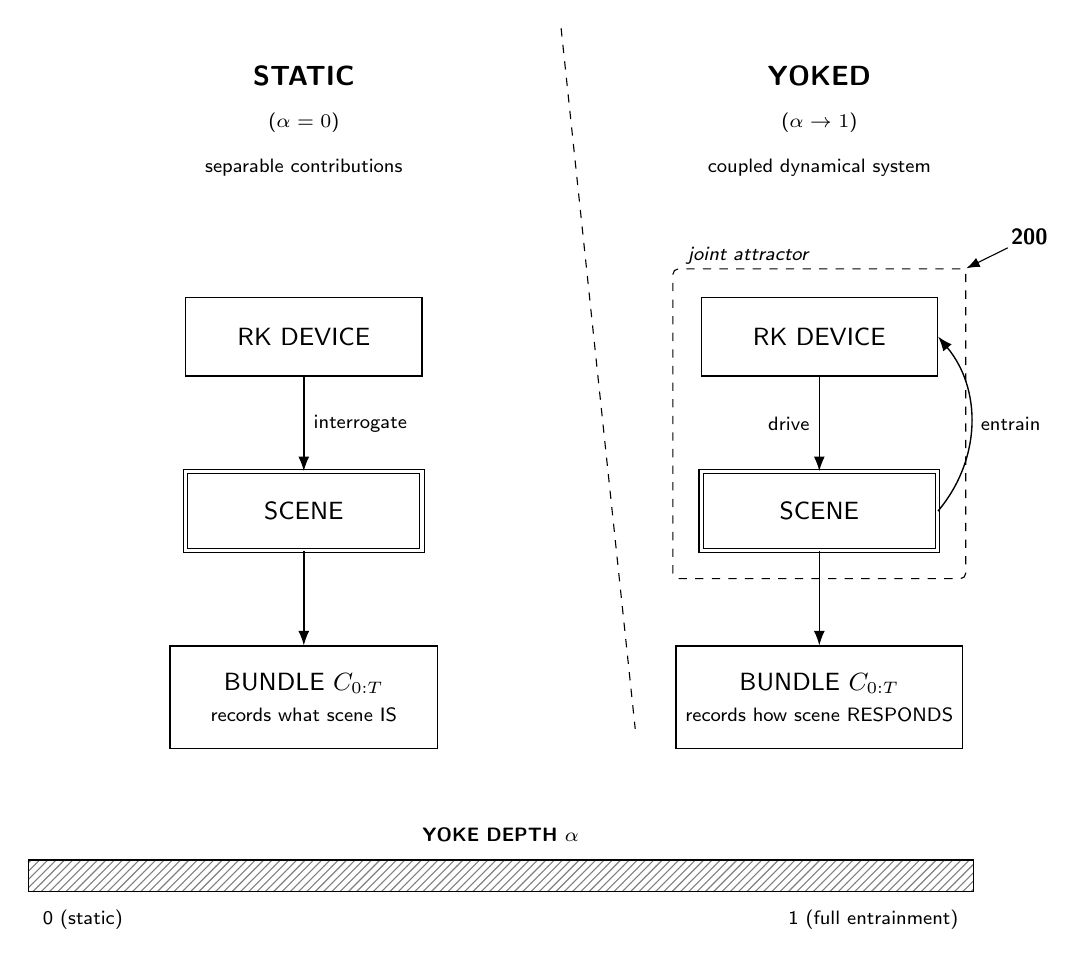
\begin{tikzpicture}[node distance=8mm]

% ============== LEFT: STATIC (alpha = 0) ==============
\node[font=\bfseries] (lhdr) at (0,0) {STATIC};
\node[font=\scriptsize, below=1mm of lhdr] (lhdr2) {($\alpha = 0$)};
\node[font=\scriptsize, below=1mm of lhdr2] (lhdr3) {separable contributions};

\node[cbox, below=14mm of lhdr3, minimum width=3cm] (lrk) {RK DEVICE};
\node[scenebox, below=12mm of lrk, minimum width=3cm] (lscene) {SCENE};
\node[cbox, below=12mm of lscene, minimum width=3.4cm, minimum height=1.3cm] (lbundle) {BUNDLE $C_{0:T}$\\\scriptsize records what scene IS};

\draw[flowarr] (lrk.south) -- node[right] {interrogate} (lscene.north);
\draw[flowarr] (lscene.south) -- (lbundle.north);

% ============== Vertical separator ==============
\draw[line width=0.4pt, dashed] ($(lhdr.east)+(2.5cm,0.6cm)$) -- ($(lbundle.east)+(2.5cm,-0.4cm)$);

% ============== RIGHT: YOKED (alpha -> 1) ==============
\node[font=\bfseries, right=5cm of lhdr] (rhdr) {YOKED};
\node[font=\scriptsize, below=1mm of rhdr] (rhdr2) {($\alpha \to 1$)};
\node[font=\scriptsize, below=1mm of rhdr2] (rhdr3) {coupled dynamical system};

\node[cbox, below=14mm of rhdr3, minimum width=3cm] (rrk) {RK DEVICE};
\node[scenebox, below=12mm of rrk, minimum width=3cm] (rscene) {SCENE};
\node[cbox, below=12mm of rscene, minimum width=3.4cm, minimum height=1.3cm] (rbundle) {BUNDLE $C_{0:T}$\\\scriptsize records how scene RESPONDS};

\draw[flowarr] (rrk.south) -- node[left] {drive} (rscene.north);
\draw[flowarr] (rscene.east) to[bend right=40] node[right, font=\scriptsize] {entrain} (rrk.east);
\draw[flowarr] (rscene.south) -- (rbundle.north);

% Joint-attractor enclosure 200
\begin{scope}[on background layer]
  \node[enclosure, fit=(rrk)(rscene), inner sep=10pt] (joint) {};
\end{scope}
\node[font=\scriptsize\itshape, anchor=south west] at ($(joint.north west)+(2pt,-2pt)$) {joint attractor};
\node[refnum] at ($(joint.north east)+(8mm,4mm)$) (n200) {\textbf{200}};
\draw[leader] (n200.south west) -- (joint.north east);

% ============== Yoke depth alpha axis ==============
\node[draw, line width=0.4pt, pattern=north east lines, pattern color=black!50,
      below=14mm of lbundle, xshift=2.5cm, minimum width=12cm, minimum height=4mm] (axis) {};
\node[font=\scriptsize\bfseries, above=1mm of axis] {YOKE DEPTH $\alpha$};
\node[font=\scriptsize, anchor=north west] at ($(axis.south west)+(2pt,-1mm)$) {0 (static)};
\node[font=\scriptsize, anchor=north east] at ($(axis.south east)+(-2pt,-1mm)$) {1 (full entrainment)};

\end{tikzpicture}
\end{center}

\end{document}
